\chapter{Introduction}\label{chap:introduction}

\section{Motivation}

This chapter demonstrates a traditional dissertation chapter. Use separate
files for each chapter so the main file remains short and easy to maintain.
LaTeX handles numbered sections, cross-references, citations, and lists of
figures and tables. For example, Figure~\ref{fig:example-main} and
Table~\ref{tab:example-main} are numbered within Chapter~\ref{chap:introduction}.

\lipsum[2]

\begin{figure}[htbp]
  \centering
  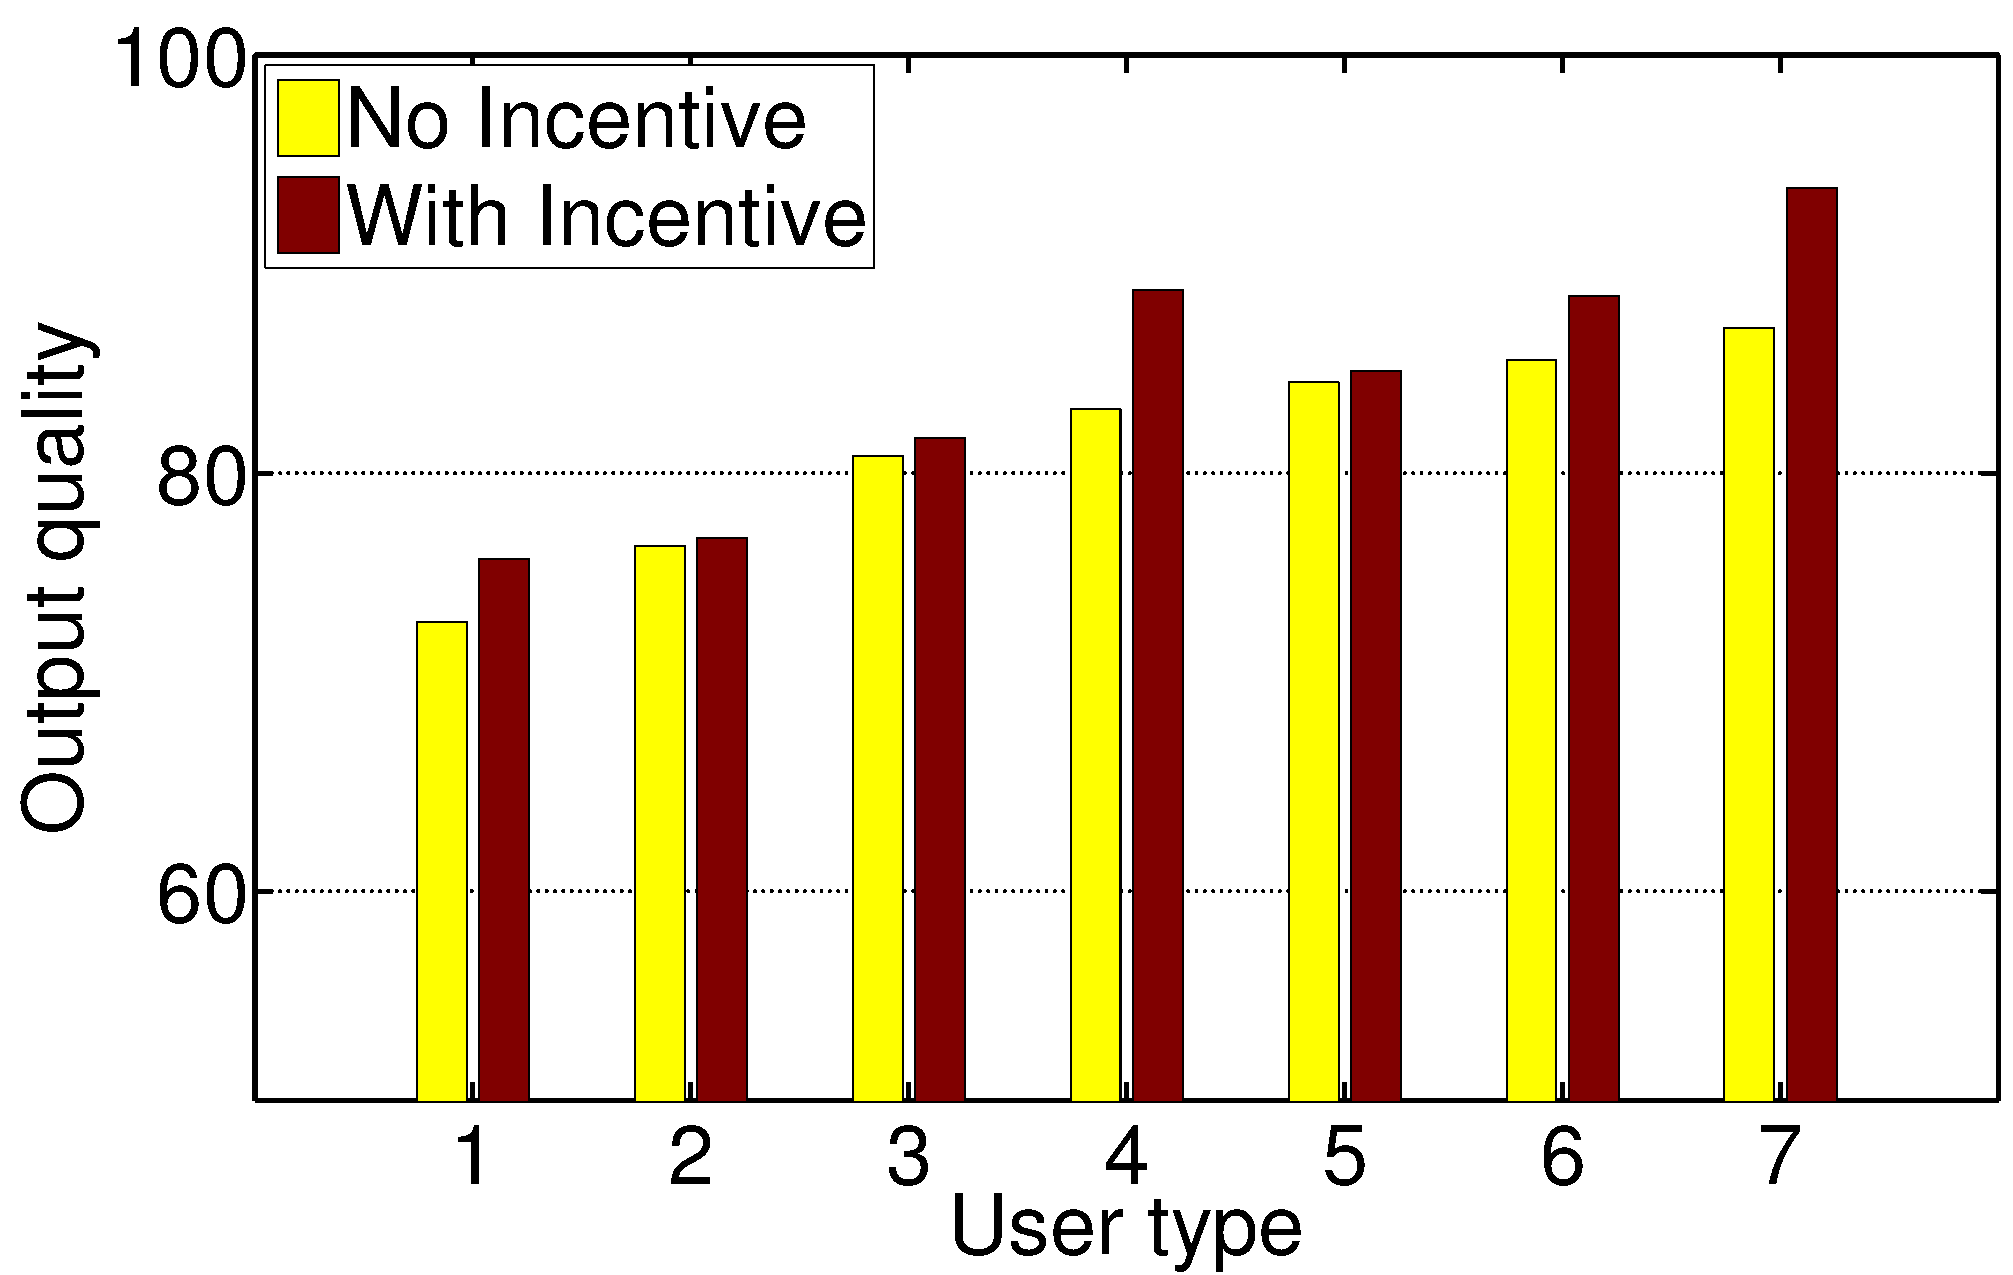
\includegraphics[width=0.75\linewidth]{fig1}
  \caption{Example figure in the main dissertation text.}
  \label{fig:example-main}
\end{figure}

\section{Example Table}

\begin{table}[htbp]
  \caption{Example table using booktabs.}
  \label{tab:example-main}
  \centering
  \begin{tabular}{ll}
    \toprule
    Element & Purpose \\
    \midrule
    Chapters & Main dissertation text \\
    Appendices & Supporting information or supplemental material \\
    References & Bibliography generated from a BibTeX file \\
    \bottomrule
  \end{tabular}
\end{table}

\section{Citations}

This template uses BibTeX and natbib. Parenthetical citations can be written as
\citep{goossens1994latex}; textual citations can be written as
\citet{lamport1994latex}.
